\begin{tikzpicture}[
    grow'=right,
    sloped,
    level distance=3.5cm,
    sibling distance=1cm,
    align=center,
    anchor=north
]
% \tikzset{every tree node/.style={align=center,anchor=north}}
\Tree
[.{}
    \edge node[midway, above] {$0{,}45$};
    [.$A$
        \edge node[midway, above] {$0{,}85$}; [.$R$ ]
        \edge node[midway, below] {$0{,}15$}; [.$\bar{R}$ ]
    ]
    \edge node[midway, above] {$0{,}10$};
    [.$B$
        \edge node[midway, above] {$0{,}84$}; [.$R$ ]
        \edge node[midway, below] {$0{,}16$}; [.$\bar{R}$ ]
    ]
    \edge node[midway, below] {$0{,}03$};
    [.$AB$
        \edge node[midway, above] {$0{,}82$}; [.$R$ ]
        \edge node[midway, below] {$0{,}18$}; [.$\bar{R}$ ]
    ]
    \edge node[midway, below] {$0{,}42$};
    [.$O$
        [.$R$ ]
        [.$\bar{R}$ ]
    ]
]
\end{tikzpicture}